%%This is a very basic article template.
%%There is just one section and two subsections.
\documentclass[a4paper,11pt]{scrartcl}
\usepackage{polski}
\usepackage[utf8]{inputenc}
\usepackage[T1]{fontenc}
\usepackage{datetime}

\usepackage{listings}
\usepackage{graphicx, graphics, epsfig, geometry, pslatex}
\usepackage{amsmath, amssymb}
\usepackage{url}

\usepackage{array}
\usepackage{times}
\usepackage{caption}
\usepackage{a4wide}
\usepackage{units}

\newcommand{\figsource}[1]{
\captionsetup{font={scriptsize, it}}
\caption*{Źródło: \url{#1}}
\captionsetup{font={normalsize}}
}

\newcommand{\f}{\texttt}
\newcommand{\mytitlea}{Peer-to-peer web objects}
\newcommand{\mytitleb}{caching proxy}
\newcommand{\me}{Tomasz Drwięga}
\newcommand{\s}{ }

\newcommand{\kesz}{cache}
\newcommand{\keszy}{cache'y}
\newcommand{\kesza}{cache'a}
\newcommand{\keszowi}{cache'owi}
\newcommand{\keszem}{cache'em}
\newcommand{\keszu}{cache'u}
\newcommand{\keszujace}{cache'ujące}
\newcommand{\keszujacego}{cache'ującego}
\newcommand{\keszujacy}{cache'ujący}
\newcommand{\keszujacym}{cache'ującym}
\newcommand{\keszujacych}{cache'ujących}
\newcommand{\keszowania}{cache'owania}
\newcommand{\keszowanie}{cache'owanie}
\newcommand{\keszowaniem}{cache'owaniem}

\lstset{numbers=left,
	numberstyle=\tiny,
	%basicstyle=\footnotesize,
	showstringspaces=false,
	basicstyle=\footnotesize,
	breaklines=true,
	captionpos=b,
	tabsize=3,
	stepnumber=60,
	firstnumber=1,
	}
%opening
\title{\mytitlea \mytitleb}
\author{\me}

\makeindex

\begin{document}

% \parindent0pt
\pagestyle{empty}

\begin{titlepage}
\vspace*{\fill}
\begin{center}
\begin{picture}(300,510)
	\put( 0,520){\makebox(0,0)[l]{\large \bf \textsc{Wydział Podstawowych
	Problemów Techniki}}}
	\put( 0,500){\makebox(0,0)[l]{\large \bf \textsc{Politechniki Wrocławskiej}}}
	\put(15,280){\makebox(0,0)[l]{\Huge  \bf \textsc{\mytitlea}}}
	\put(80,250){\makebox(0,0)[l]{\Huge  \bf \textsc{\mytitleb}}}
	\put(95,220){\makebox(0,0)[l]{\Large     \textsc{\me}}}
	
	\put(190, 80){\makebox(0,0)[l]{\large  {Praca magisterska napisana}}}
	\put(190, 60){\makebox(0,0)[l]{\large  {pod kierunkiem}}}
	\put(190, 40){\makebox(0,0)[l]{\large  {dra Mirosława Korzeniowskiego}}}
	
	\put(110,-80){\makebox(0,0)[bl]{\large \bf \textsc{Wrocław 2013}}}
\end{picture}
\end{center}
\vspace*{\fill}
\end{titlepage}

\tableofcontents

\newpage

\pagestyle{headings}

\section*{Wstęp}

TODO: Opis problemu cachowania (oryginalnego - hot spots), nasilenie związane z efektem slash-dot, multimedia

\section{Historia \keszowania}
Wraz z rosnącą liczbą użytkowników Internetu w latach dziewięćdziesiątych zaczęły pojawiać się problemy z dostępem do pewnych zasobów.
Duża liczba odwołań do popularnych stron w krótkim czasie powodowała znaczące obciążenie serwerów, które dany zasób posiadały.
Czasami z powodu nadmiernego zalania\footnote{ang. \textit{flooded}, \textit{swamped}} żądaniami serwer nie był w stanie obsłużyć wszystkich, przez co strona stawała się niedostępna.

\subsection{Serwery \keszujace}\label{sect_cache}
Jako rozwiązanie problemu ,,gorących punktów'' (ang. \textit{hot spots}) pojawiły się serwery \keszujace. Rysunek \ref{fig_cache_server} przedstawia wprowadzenie transparentnego, lokalnego \kesza\s i jego relację z serwerem docelowym. 
Żądania zasobów wychodzące od użytkowników końcowych są w pierwszej kolejności obsługiwane przez serwer \keszujacy, który odpowiada zapamiętanym zasobem lub kontaktuje się z serwerem docelowym i zapamiętuje odpowiedź.

\begin{figure}[ht]
\centering
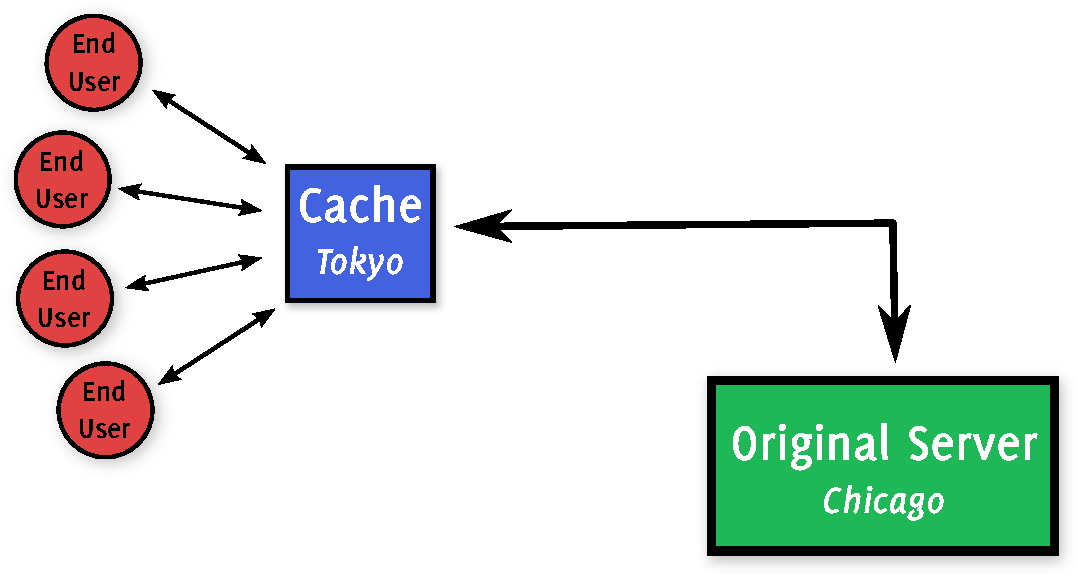
\includegraphics[width=0.85\linewidth]{img/cache.pdf}
\caption{
Przykład lokalnego serwera \keszujacego.
Zamiast wielokrotnie odwoływać się do docelowego serwera, który zawiera daną stronę
możemy zapamiętać ją na serwerze \keszujacym. Takie rozwiązanie niesie ze sobą zalety
zarówno dla administratorów serwera w Chicago, jak i użytkowników sieci w Japonii:
mniej żądań skutkuje mniejszym obciążeniem serwera, a ,,lokalność'' serwera \keszujacego\s zmniejsza opóźnienia i zwiększa szybkość transferu zasobu.
}
\label{fig_cache_server}
\end{figure}

Wprowadzenie \keszowania\s niesie ze sobą szereg zalet nie tylko dla administratorów serwerów zawierających zasoby. Serwery znajdujące się na granicy sieci lokalnej z Internetem (jak na rysunku \ref{fig_cache_server}) oferują użytkownikom tej sieci lepszy transfer i mniejsze opóźnienia w dostępie do popularnych zasobów.
Ponieważ łącze wychodzące z sieci ma ograniczoną przepustowość, \kesz\s pozwala również na jego oszczędniejsze wykorzystanie, a tym samym poprawę jakości dostępu do Internetu.

\subsection{Rozproszony i hierarchiczny \kesz}\label{sect_dist_cache}
Rozwiązanie przedstawione w rozdziale \ref{sect_cache} pozwala na odciążenie serwera docelowego. Zastanówmy się jednak co będzie się działo w przypadku zwiększania liczby użytkowników korzystających z serwera \keszujacego. Duża liczba żądań może spowodować dokładnie taką samą sytuację jak w przypadku serwera docelowego - \kesz\s zostanie zalany i nie będzie w stanie obsłużyć wszystkich zapytań.

W 1995 roku Malpani i inni \cite{malpani1995making} zaproponowali metodę, w której wiele serwerów \keszujacych\s współpracuje ze sobą w celu zrównoważenia obciążenia. W ich propozycji klient wysyła żądanie do losowego serwera należącego do systemu. W przypadku, gdy serwer posiada określony zasób odsyła go w odpowiedzi, w przeciwnym razie rozsyła to żądanie do wszystkich innych serwerów. Jeżeli żaden z \keszy nie zawiera zasobu, to żądanie jest przesyłane do serwera oryginalnego. Niestety wraz ze wzrostem liczby serwerów, należących do systemu liczba przesyłanych między nimi wiadomości bardzo szybko rośnie i cały system staje się zawodny.

W ramach projektu Harvest \cite{bowman1994harvest} A. Chankhunthod i inni \cite{chankhunthod1995hierarchical} stworzyli \kesz\s hierarchiczny. Rozwiązanie to pozwala łączyć kilka serwerów w system, który można skalować w zależności od liczby użytkowników, których ma obsługiwać. Grupy użytkowników łączą się z serwerami, będącymi liśćmi. Przychodzące żądania są obsługiwane najpierw przez serwery na najniższym poziomie, w przypadku gdy te serwery nie mają danego zasobu w \keszu\s decydują czy pobrać go z serwera docelowego, czy odpytać serwery z tego samego i wyższego poziomu. Decyzja podejmowana jest na podstawie opóźnień do obu serwerów.

\begin{figure}[h]
\centering
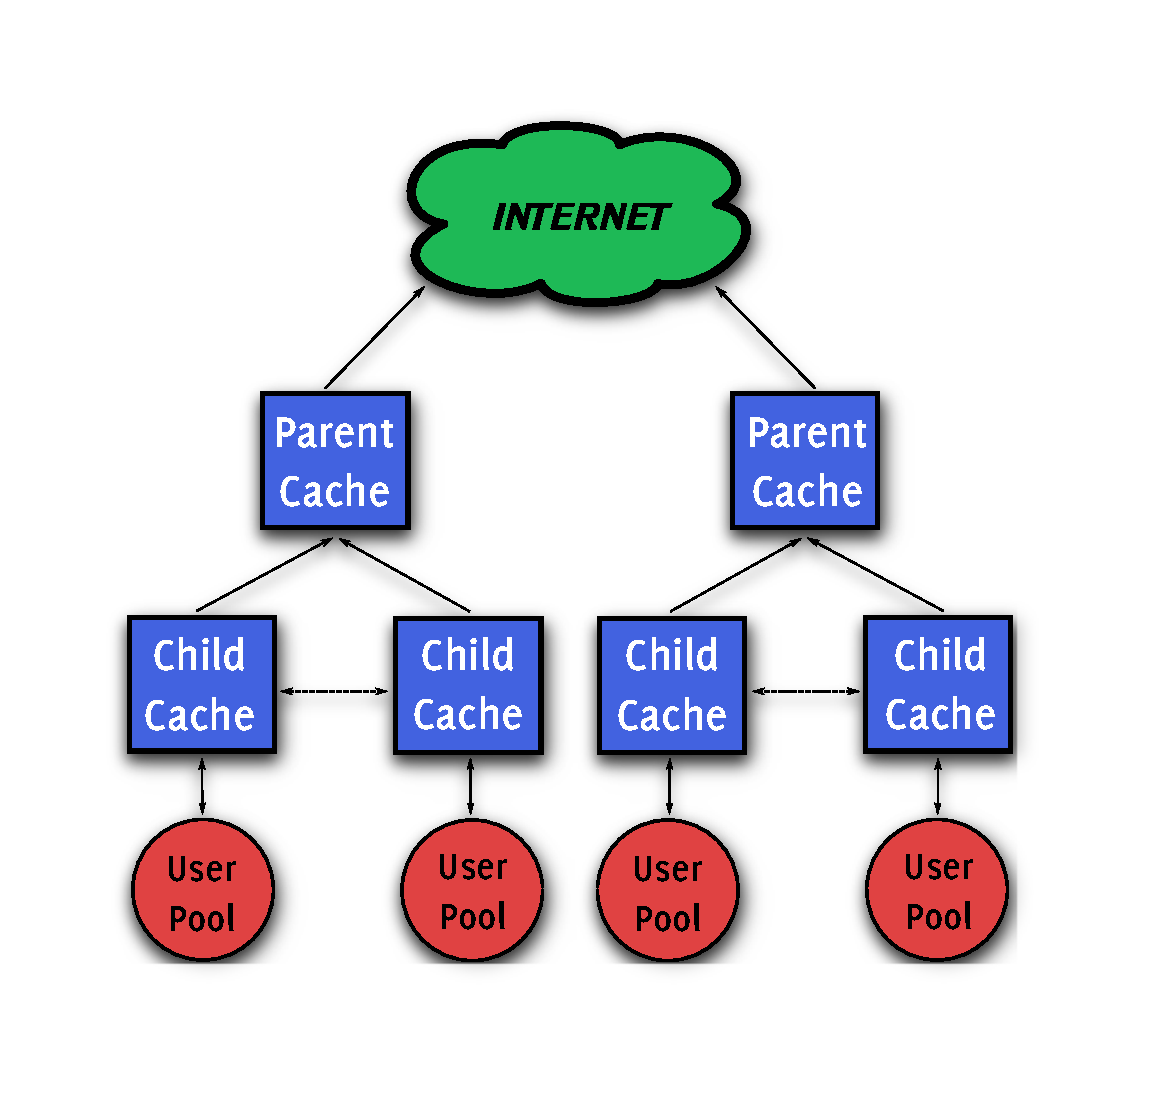
\includegraphics[width=0.8\linewidth]{img/hierarchical.pdf}
\label{fig_cache_hierarchical}
\caption{Połączenie kilu serwerów \keszujacych\s w system hierarchiczny. Każdy z serwerów znajdujących się w liściach obsługuje określoną liczbę użytkowników. Zapytania o zasoby, które nie znajdują się w \keszu\s wysyłane są do rodzica.}
\end{figure}

W praktyce, w takim systemie serwery na wyższych poziomach muszą obsługiwać dużą liczbę żądań od dzieci przez co stają się wrażliwe na zalanie oraz składują duże ilości danych \cite{povey1997distributed}.

Kolejnym zaproponowanym udoskonaleniem jest \kesz\s rozproszony. Rozwiązanie zachowuje hierarchiczną strukturę w formie drzewa, ale tym razem jedynie serwery w liściach zajmują się \keszowaniem\s zasobów, a pozostałe serwery stanowią indeks, w którym zapamiętywana jest informacja czy zasób znajduje się w systemie oraz jaki serwer go przechowuje.

Jak pokazały eksperymenty \cite{povey1997distributed} rozproszony \kesz\s oferuje zbliżoną wydajność do \keszu\s hierarchicznego rozwiązując dodatkowo problemy związane z obsługą dużej liczby żądań przez serwery na wyższych poziomach.

\subsection{Dynamiczna restrukturyzacja}
Przedstawione w rozdziałach \ref{sect_cache} i \ref{sect_dist_cache} metody \keszowania\s nie są przystosowane do działania w warunkach, w którym obciążenie czy liczba użytkowników obsługiwanych przez system się zmienia. Wraz z rosnącą liczbą żądań nie jest możliwe łatwe poprawienie wydajności przez dołożenie dodatkowych serwerów \keszujacych. Wprowadzenie zmian w systemie wymaga zmian w konfiguracji poszczególnych serwerów. Dodatkowo awarie pojedynczych węzłów mogą spowodować nieprawidłową pracę \keszu.

W celu ułatwienia dodawania i usuwania serwerów do systemu możemy spróbować innego podejścia do problemu. Podstawowym zadaniem węzłów wewnętrznych w systemie \keszu\s rozproszonego jest utrzymywanie indeksu przechowywanych zasobów i lokalizacja serwera, który dany zasób obsługuje. Zatem jeżeli klient mógłby określić, który serwer \keszujacy\s jest odpowiedzialny za obsługę obiektu, wtedy cała infrastruktura związana z indeksowaniem byłaby niepotrzebna.

Naiwnym rozwiązaniem stosującym takie podejście jest przypisanie zasobów do konkretnych serwerów. Przyjmijmy za identyfikator zasobu jego adres. Możemy teraz przypisać wszystkie zasoby w obrębie jednej domeny do pewnego serwera. Na przykład dysponując 24 serwerami możemy przypisać wszystkie domeny zaczynające się na ,,a'' do serwera pierwszego, na ,,b'' do drugiego itd. Oczywiście pozwoli to na łatwe określenie, który serwer należy odpytać o dany zasób, ale rozwiązanie to ma dwie poważne wady. Po pierwsze rozwiązanie nie jest skalowalne - niezdefiniowane jest jakie zasoby miałby obsługiwać dodatkowy serwer, a po drugie obciążenie na serwerach jest nierównomierne.

Możemy jednak spróbować rozwiązać problem przydziału zasobów do serwerów nieco inaczej. Niech $n$ oznacza liczbę serwerów, a $R$ adres pewnego zasobu, wtedy:
\begin{equation*}
S \equiv hash(R) \bmod n,
\end{equation*}
 gdzie $S$ oznacza indeks serwera odpowiedzialnego za zasób $R$, a $hash$ jest funkcją haszującą. Dzięki właściwościom funkcji haszujących gwarantujemy, że zasoby każdy z serwerów jest odpowiedzialny za równą część składowanych zasobów. Niestety dalej nie jest rozwiązany problem skalowalności. Dodanie $n+1$ serwera powoduje, że wszystkie zasoby zostaną przypisane w inne miejsca.
 
\subsubsection{\textit{Consistent Hashing}}
\label{sect_consistent_hashing}
Podczas dodawania nowego serwera do systemu oczekujemy, że przejmie on od pozostałych równą część zasobów, aktualnie znajdujących się w \keszu. Dodatkowo nie chcemy, aby wartości w \keszu były przesuwane pomiędzy ,,starymi'' serwerami. Taką własność gwarantuje mechanizm \textit{Consistent Hashing}, opracowany przez Kargera i Lehmana \cite{karger1997consistent}.

Załóżmy, że dysponujemy funkcją haszującą w odcinek $[0, 1]$, za pomocą której każdemu zasobowi i serwerowi przyporządkowujemy punkt na tym odcinku. Dodatkowo, traktujemy odcinek jako okrąg o obwodzie równym 1. W podanym przez Kargera i Lehmana schemacie dany zasób jest obsługiwany przez najbliższy serwer idąc zgodnie z ruchem wskazówek zegara. Rysunek \ref{fig_consistent_hashing} przedstawia przykładowe mapowanie zasobów i ich przyporządkowanie do poszczególnych serwerów. W drugiej części rysunku przedstawiona została zmiana przyporządkowania wynikająca z dodania nowego serwera $D$.

\begin{figure}[ht]
\centering
\begin{minipage}[b]{0.445\linewidth}
\centering
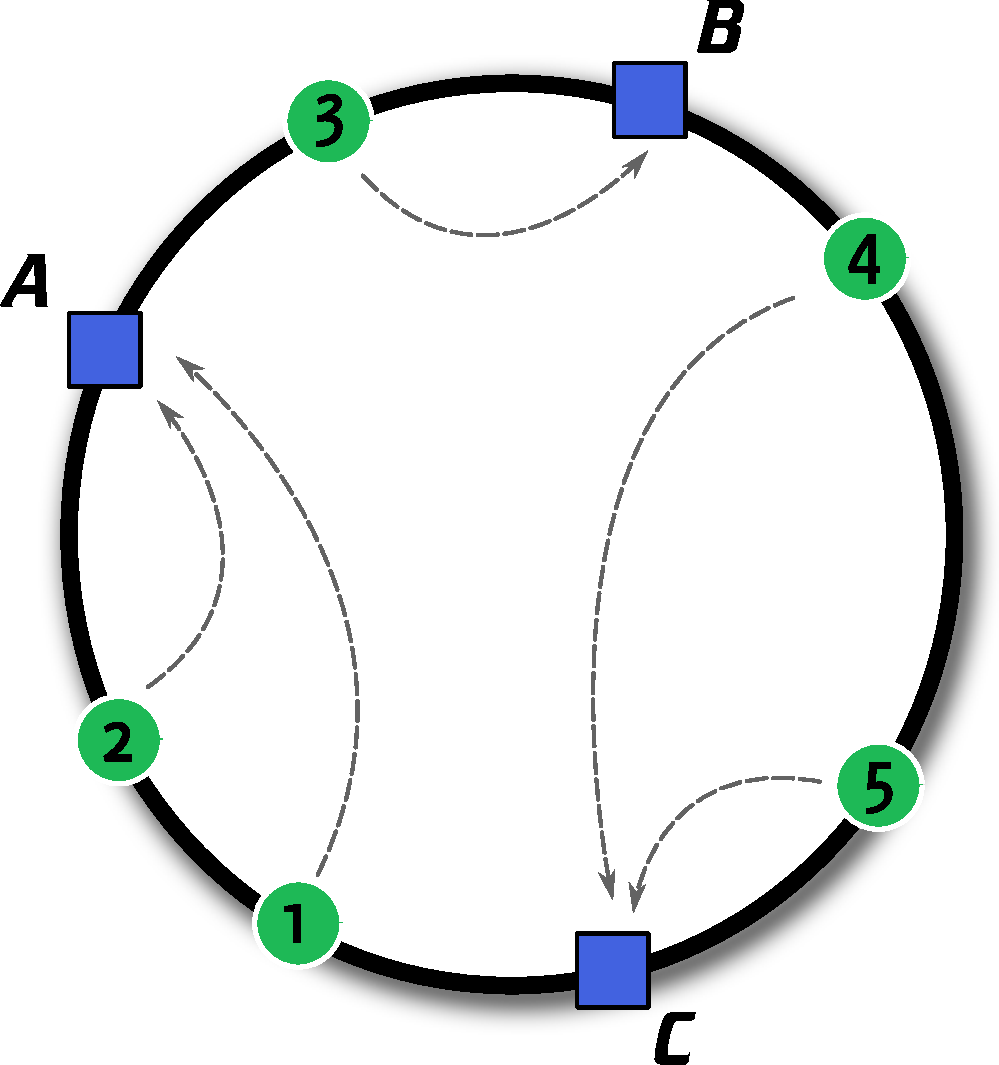
\includegraphics[width=0.95\textwidth]{img/consistent.pdf}
\end{minipage}
\begin{minipage}[b]{0.47\linewidth}
\centering
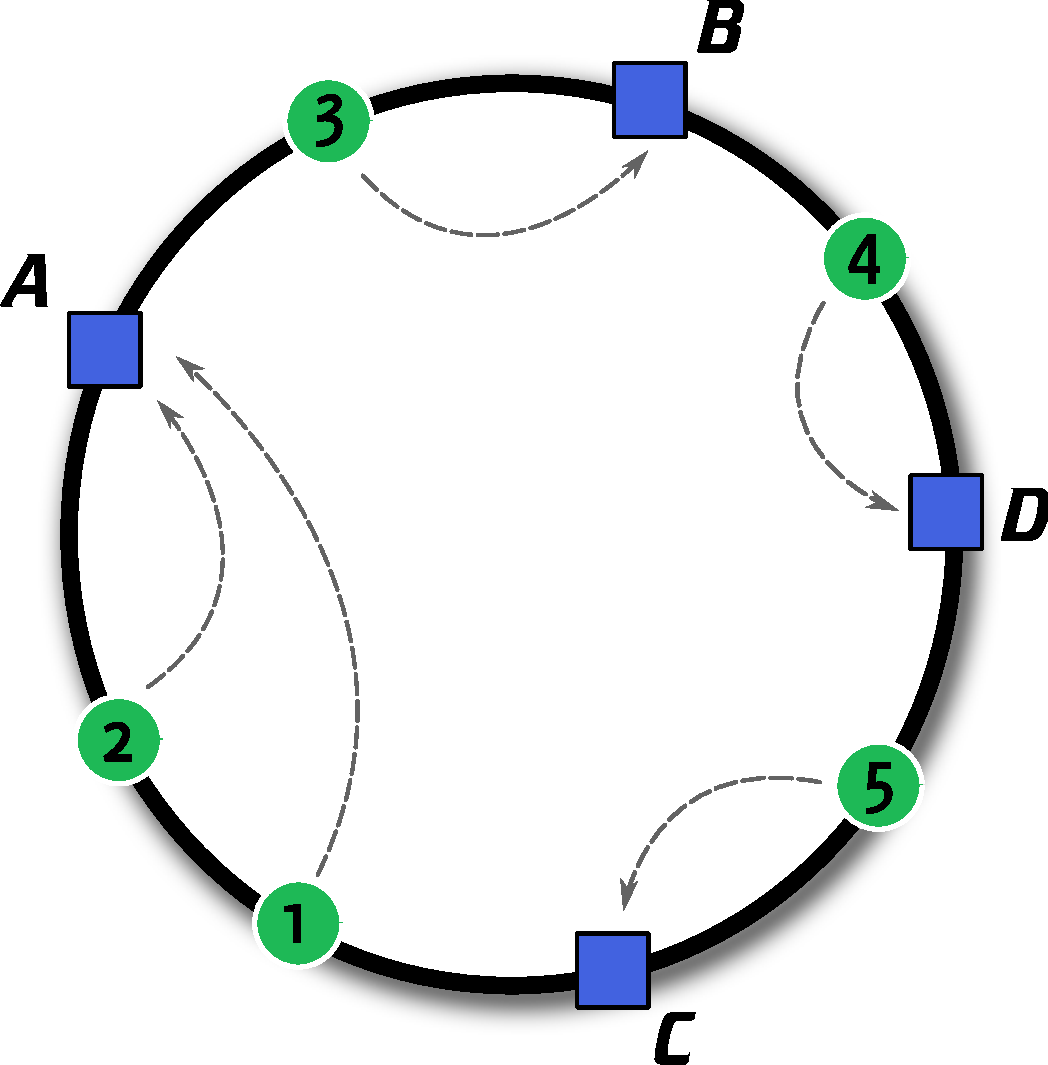
\includegraphics[width=0.95\textwidth]{img/consistent_2.pdf}
\end{minipage}
\caption{Idea \textit{Consistent Hashing}. Zasoby, reprezentowane przez zielone punkty, oraz serwery \keszujace\s (kwadraty) mapowane są na punkty na okręgu o jednostkowym obwodzie. W praktyce do reprezentowania punktów na okręgu najczęściej wykorzystywane są klucze binarne o ustalonej długości $m$. Każdy serwer jest odpowiedzialny za obsługę zasobów znajdujących się pomiędzy jego punktem i punktem jego poprzednika. Dodanie nowego serwera $D$ powoduje wyłącznie zmianę przydziału zasobu $4$.}
\label{fig_consistent_hashing}
\end{figure}

W praktyce, przesłanie informacji dotyczących zmian serwerów do wszystkich klientów byłoby bardzo kosztowne, ale sytuacja, w której klienci mają różne ,,widoki'' (wiedzą tylko o pewnym podzbiorze serwerów) systemu nie stanowi problemu po wprowadzeniu prostej modyfikacji. Zauważmy, że może dojść do sytuacji, w której jeden z serwerów, z powodu niepełnej wiedzy klientów, będzie obsługiwał więcej żądań od pozostałych. W celu rozwiązania nierównego obciążenia autorzy zaproponowali stworzenie wirtualnych kopii serwerów, tzn. każdy z nich zmapowany jest nie do jednego, lecz kilku punktów na okręgu. Dzięki temu zagwarantowane jest równomierne przyporządkowanie zasobów do serwerów \cite{karger1999web}.

Pomimo, że pierwotną motywacją powstania \textit{Consistent Hashing} był problem \keszowania\s zasobów internetowych, schemat znalazł zastosowanie w innych obszarach. W szczególności, leży on u podstaw rozproszonych tablic haszujących, które omówione są w rozdziale \ref{sect_dht}.

\section{Rozproszone tablice haszujące (DHT)}
\label{sect_dht}
Rozproszone tablice haszujące (ang. \textit{Distributed Hash Tables}, DHT) to systemy pozwalające na przechowywanie par \textit{(klucz, wartość)}, podobnie jak zwykłe tablice haszujące, w dynamicznej sieci zbudowanej z uczestniczących węzłów (\textit{peer-to-peer}). Odpowiedzialność za przetrzymywanie mapowania kluczy do wartości jest podzielona pomiędzy węzły, w taki sposób aby zmiany w liczbie uczestników nie powodowały reorganizacji całości systemu, ale tylko jego drobnej części. Dodatkowo rozproszone tablice haszujące oferują efektywne wyszukiwanie kluczy w systemie.

Początkowe badania nad DHT były motywowane istniejącymi systemami peer-to-peer, oferującymi głównie możliwość dzielenia się plikami, np. \textit{Napster}, \textit{Gnutella} i \textit{Freenet}. Sieci te na różne sposoby realizowały wyszukiwanie zasobów, ale każdy z nich miał swoje wady. \textit{Napster} korzystał z centralnego katalogu, do którego każdy serwer wysyłał swoją listę plików i który zarządzał wyszukiwaniem plików. W \textit{gnutelli} w celu odnalezienia zasobu, zapytanie wysyłane było do każdego węzła w sieci w określonym promieniu, co skutkowało mniejszą szybkością i mnóstwem przesyłanych wiadomości oraz podobnie jak w przypadku sieci \textit{Freenet}, w której znajdowanie klucza odbywało się za pomocą heurystycznej metody, brak gwarancji odnalezienia klucza.

Idea rozproszonych tablic haszujących ma na celu rozwiązanie wszystkich przedstawionych problemów:
\begin{itemize}
  \item w pełni rozproszony, skalowalny system; brak centralnego zarządzania,
  \item odporność na awarie węzłów,
  \item deterministyczny algorytm routingu, z dowiedzioną poprawnością, pozwalający na efektywne wyszukiwanie. 
\end{itemize} 

Jedną z pierwszy sieci DHT, bazującej na schemacie \textit{Consistent Hashing} jest \textit{Chord}, opisany w rozdziale \ref{sect_dht_chord}.

\subsection{Chord}
\label{sect_dht_chord}
Sieć \textit{Chord} opracowana przez Stoicę, Morrisa, Kargera, Kaashoeka i Balakrishnana  \cite{stoica2001chord} to jedna z czterech pierwszych powstałych rozproszonych tablic haszujących\footnote{Pozostałe to CAN\cite{ratnasamy2001scalable}, Tapestry \cite{zhao2001tapestry} i Pastry\cite{rowstron2001pastry}.}. Zapewnia szybki i odporny na błędy protokół routingu, znajdujący węzeł odpowiedzialny za dany klucz w czasie logarytmicznym w stosunku do liczby węzłów w sieci.

U podstaw \textit{Chorda} leży mechanizm \textit{Constistent Hashing} opisany w rozdziale \ref{sect_consistent_hashing}. W przypadku \textit{Constistent Hashing}, aby zlokalizować węzeł odpowiedzialny za dany klucz wymagana była znajomość wszystkich węzłów w sieci. Takie rozwiązanie pozwala na szybkie odnalezienie węzła, ale nie daje możliwości skalowania na dowolną liczbę węzłów. W uproszczonej wersji \textit{Chorda}, w celu zapewnienia efektywnego skalowania, autorzy wymagają wyłącznie znajomości przez węzeł swojego następnika. Dzięki temu, niezależnie od wielkości sieci każdy z węzłów przechowuje informacje tylko o jednym sąsiedzie, ale czas odnalezienia dowolnego klucza jest liniowy w stosunku do liczby węzłów (wiadomości są przesyłane po pierścieniu aż dotrą do docelowego serwera).

\begin{figure}[h]
\centering
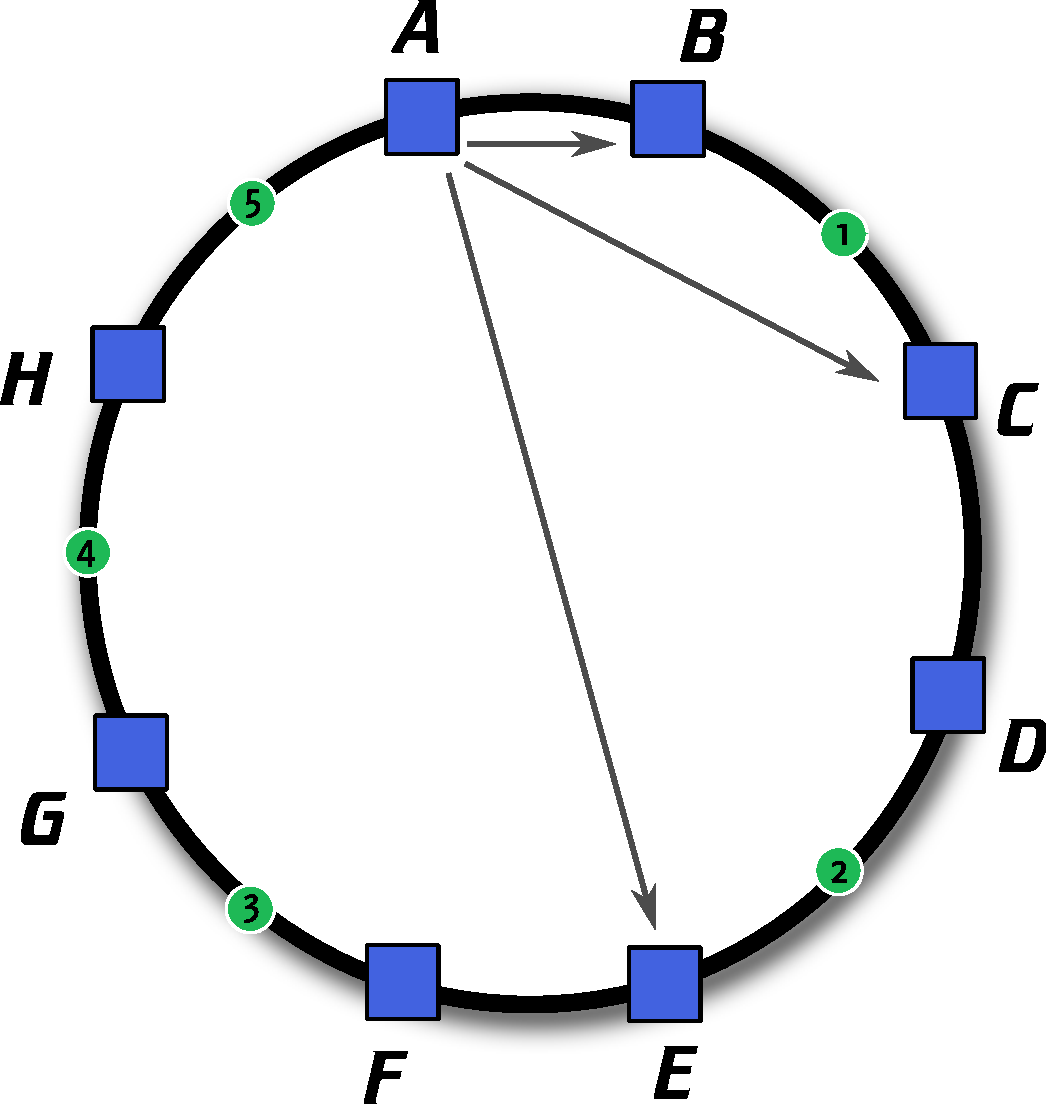
\includegraphics[width=0.5\linewidth]{img/chord.pdf}
\caption{Kontakty (\textit{fingers}) węzła $A$ w sieci Chord. Dla ustalonej długości klucza $m$, węzeł $n$ przechowuje kontakty: $successor(n + 2^{i-1})$ dla każdego $i = 1, 2, \dots,  m$; gdzie $successor(k)$ oznacza serwer odpowiedzialny za klucz $k$.}
\label{fig_chord_fingers_1}
\end{figure}

Bardziej efektywna wersja routingu zakłada, że każdy z węzłów utrzymuje tabelę z kontaktami w określonych odległościach od niego samego. Kolejne kontakty są wykładniczo coraz bardziej odległe tak, jak przedstawione to zostało na rysunku \ref{fig_chord_fingers_1}. Takie podejście pozwala na odnalezienie węzła odpowiedzialnego za zadany klucz w czasie $O (\log n)$. Aby łatwiej zauważyć tę własność, możemy przedstawić kontakty w formie drzewa (rysunek \ref{fig_chord_fingers_2}). Każdy krok w routingu \textit{Chorda} skraca wtedy pozostały dystans co najmniej o połowę.


\begin{figure}[h]
\centering
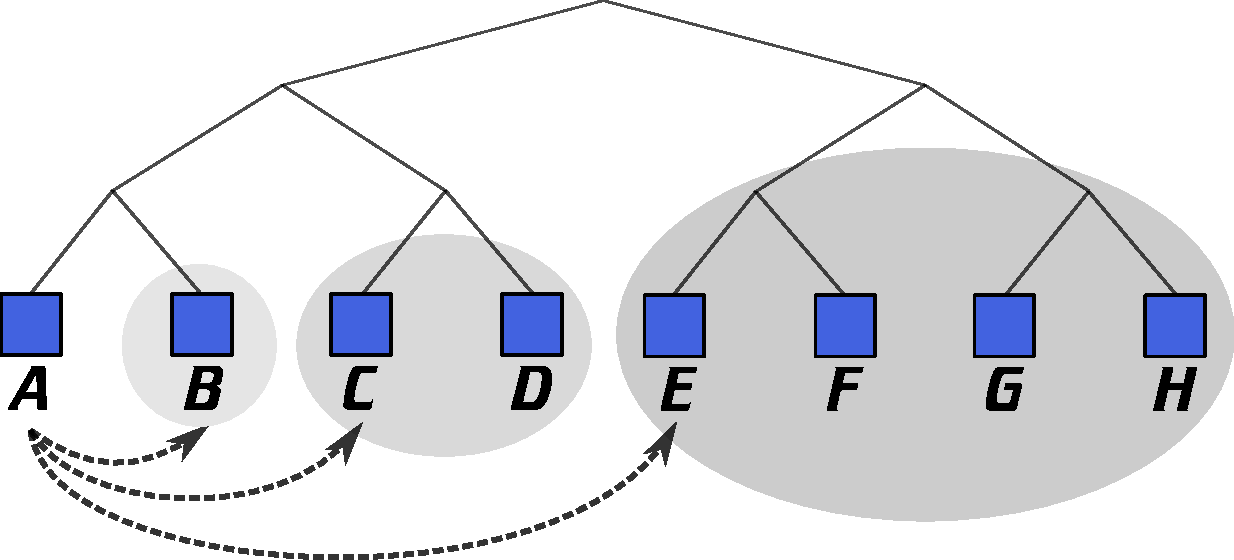
\includegraphics[width=0.9\linewidth]{img/chord_2.pdf}
\caption{Kontakty węzła $A$ w sieci Chord w postaci drzewa. Węzeł ma możliwość kontaktowania się z pojedynczymi węzłami w kolejnych poddrzewach, o co raz większej wysokości.  
TODO: Pełniejszy opis i powiązanie z Kademlią?}
\label{fig_chord_fingers_2}
\end{figure}

Podczas dołączania do sieci węzeł $n$ musi znać adres co najmniej jednego węzła, który należy już do sieci, nazwijmy go $n'$. Procedura dołączania polega na poproszeniu $n'$ o znalezienie następnika dla $n$. W kolejnym kroku $n$ buduje tablicę kontaktów wysyłając zapytania o $successor(n + 2^{i-1})$ dla każdego kolejnego $i$. Po zakończeniu tego procesu $n$ posiada pełną listę kontaktów, ale tylko jego następnik wie o jego istnieniu.

TODO: kolejny akapit jest gówniany, bo nagle z dupy zaczyna rzucać jakimiś procedurami.

Pozostałe węzły mają możliwość uwzględnienia nowych podczas cyklicznego wykonywania procedury $stab$??????????????TODO, odpowiadającej za uaktualnienie (poprawienie) informacji o poprzedniku i następniku dla każdego węzła. Dodatkowa procedura $fix\_fingers$, która również jest wywoływana cyklicznie, odpowiada za uaktualnianie tabel kontaktów.

\subsection{Podsumowanie}
TODO: Krótkie podsumowanie Chorda?


\subsection{Kademlia}
TODO: Opis Kademli\cite{maymounkov2002kademlia}: Routing, Asynchroniczność wywołań routingu - aspekty praktyczne.

W 2002 roku Maymounkov i Mazieres opracowali nową sieć P2P, która wykorzystywała zalety pierwszych sieci oraz uwzględniała nie tylko aspekty teoretyczne, ale również wykorzystanie sieci w praktyce.

Kademlia \cite{maymounkov2002kademlia}, podobnie jak pierwsze powstałe sieci peer-to-peer, pozwala na odnalezienie zasobu w czasie logarytmicznym od liczby węzłów w sieci. Zaletą Kademli jest fakt, że każdy pakiet wymieniany pomiędzy węzłami niesie ze sobą dodatkowe, użyteczne informacje o pozostałych węzłach, dzięki czemu nie jest konieczne wysyłanie dodatkowych komunikatów, niezbędnych do działania systemu. Wykorzystanie tej własności umożliwia użycie metryki odległości opartej na funkcji XOR, co więcej sieć pozwala na równoległe odpytywanie wielu węzłów w celu zmniejszenia opóźnień użytkownika. Szczegóły działania routingu Kademli zostały opisane w rozdziale \ref{kad_routing}.

W celu identyfikacji zasobów i węzłów w sieci Kademlia używane są 160-bitowe klucze (np. hash SHA-1 identyfikatora). Zasoby są składowane w węzłach, których klucz jest blisko identyfikatora zasobu. W celu określenia "bliskości" elementów wykorzystywana jest metryka XOR, tzn. im więcej początkowych bitów dwóch kluczy jest zgodnych tym bliżej siebie się znajdują. Dzięki temu, że funkcja XOR jest symetryczna każde zapytanie, które dociera do danego węzła, może nieść ze sobą informacje o nowym kontakcie, którym jest nadawca komunikatu.

Każdy węzeł utrzymuje swoją tablicę kontaktów wykorzystywaną podczas wyszukiwania zasobów. Tablica dla węzła o identyfikatorze $X$ składa się z $k$-pojemników (ang. \textit{$k$-buckets}), które dla każdego $i \in [0, 160)$ przechowują adresy (maksymalnie) $k$ węzłów, które znajdują się w odległości od $2^i$ do $2^{i+1}$ od danego węzła. Zatem klucze w $i$-tym pojemniku mają z $X$ wspólny prefiks długości $160 - (i+1)$, ale różnią się na bicie $160 - i$. Parametr $k$ jest stały i ustalony dla danej sieci (autorzy Kademli proponują wartość $k=20$). Na rysunku \ref{fig_kademlia} przedstawiona została przykładowa sieć dla kluczy długości $3$ oraz kontakty węzła o kluczu $000$. 

Bazując na zapisów logów zebranych przez Saroiu i innych \cite{saroiu2001measurement} z działającej sieci Gnutella, zaobserwowano, że prawdopodobieństwo, że węzeł który znajduje się w sieci od $x$ minut będzie się w niej znajdował również w czasie $x+60$ rośnie wraz ze wzrostem $x$. Własność ta została wykorzystana w Kademli w celu ustalenia kolejności w $k$-pojemnikach. Węzły są uszeregowane według malejącego czasu ostatniej widoczności\footnote{Czas ten jest uaktualniany w momencie otrzymywania zapytań lub odpowiedzi na zapytania od danego węzła.}. W momencie kiedy do danej listy ma trafić kolejny węzeł do ostatniego węzła na liście wysyłany jest komunikat w celu sprawdzenia czy jest wciąż aktywny. W przypadku braku odpowiedzi węzeł jest usuwany z listy, a nowy węzeł wstawiany jest na początek. W przeciwnym razie węzeł jest przesuwany na początek listy, a nowy kontakt jest ignorowany. Dzięki takiemu podejściu sieć dodatkowo staje się częściowo odporna na ataki, w których adwersarz wprowadza wiele nowych węzłów, które mają na celu "wypchnięcie" prawdziwych węzłów z tabel kontaktów.

\begin{figure}[h]
\centering
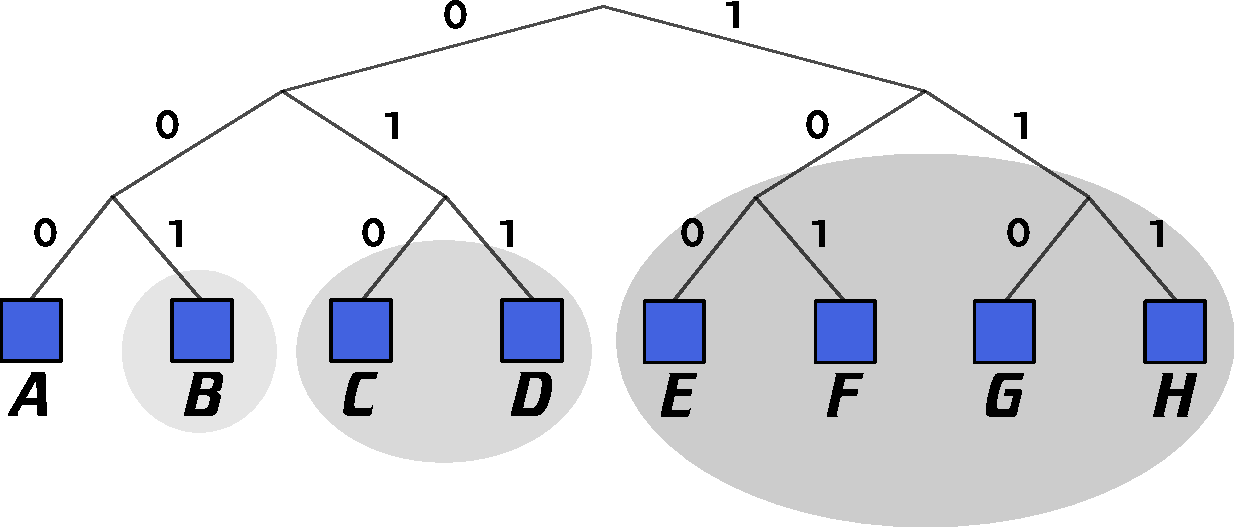
\includegraphics[width=0.9\linewidth]{img/kademlia.pdf}
\caption{Tablica kontaktów węzła $000$ w przykładowej sieci Kademli. Szare elipsy oznaczają kolejne $k$-pojemniki. Rysunek ten bardzo przypomina rysunek \ref{fig_chord_fingers_2}. W przypadku Chorda węzeł znał co najwyżej jeden węzeł z każdego poddrzewa. Dzięki zastosowaniu metryki XOR w Kademli węzły bez dodatkowych komunikatów mogą dowiedzieć się o pozostałych węzłach, które należą do danego przedziału. Informacja ta wykorzystywana jest w celu przyspieszenia routingu w praktycznych zastosowaniach.}
\label{fig_kademlia}
\end{figure}

\subsubsection{Routing}
\label{kad_routing}
Protokół Kademli oparty jest o cztery procedury: \f{STORE}, \f{PING}, \f{FIND\_NODE} oraz \f{FIND\_VALUE}. Pierwsza procedura wysyła prośbę o zapamiętanie pary (klucz, wartość). \f{PING} używany jest do ustalenia czy dany węzeł powinien zostać usunięty z pewnego $k$-pojemnika lub czy dalej jest aktywny. Dwie kolejne procedury stanowią najważniejszą część sieci. Obie używają tego samego algorytmu routingu w celu odnalezienia węzła lub wartości, która reprezentowana jest przez zadany klucz.

W celu odnalezienia węzła o kluczu $X$ przez węzeł $S$ na podstawie tablicy kontaktów określanych jest $k$ najbliższych do klucza $X$ węzłów sieci. W kolejnym kroku $S$ przesyła zapytanie o $k$ najbliższych węzłów do węzłów wybranych w poprzednim kroku. Dzięki zastosowanej metryce XOR i jej własnościom możliwe jest wysyłanie równoczesnych zapytań do kilku węzłów. Liczbę równoległych żądań określa parametr $\alpha$, dla którego Maymounkov i Mazieres proponują wartość 3. Dzięki odpytywaniu wielu węzłów w tym samym czasie możemy uzyskać krótszy czas dostępu do zasobów, w przypadku gdy część węzłów nie odpowiada na komunikaty węzła $S$. Procedura \f{FIND\_VALUE} obsługiwana jest dokładnie w ten sam sposób, dopóki jeden z węzłów nie posiada wartości odpowiadającej danemu kluczowi. Wtedy węzeł zamiast zwracać $k$ najbliższych węzłów zwraca po prostu wartość, znajdującą się pod podanym kluczem.

\subsection{Podsumowanie}
TODO: Krótkie podsumowanie kademli; Może nie robić z tego osobnego akapitu?

\section{Rozproszony \kesz\s z użyciem DHT}
Obecne zastosowania DHT skupiają się głównie na systemach wymiany plików takich jak Kad czy BitTorrent. W systemach tych DHT są używane w celu odnalezienia komputerów, które przechowują dany plik. W tej pracy proponujemy użycie DHT w celu \keszowania\s zasobów internetowych. Jak opisane zostało w rozdziale \ref{sect_consistent_hashing} \keszowanie\s zasobów leżało u podstaw powstania mechanizmu \textit{Consistent Hashing}, który z kolei zapoczątkował rozwój DHT.

\subsection{Motywacja}
Pod koniec lat dziewięćdziesiątych, kiedy opracowane zostało \textit{Constistent Hashing} z internetu korzystało 7\% światowej populacji (31\% w krajach rozwiniętych). Problemy, które stały wówczas przed twórcami mechanizmu rozpatrywane były głównie z punktu widzenia serwerów, których zalanie nadmierną liczbą zapytań powodowało czasowe problemy z dostępem do zasobów. Rozwiązania miały na celu stworzenie infrastruktury, która pozwalałaby na odciążenie serwerów i w efekcie zwiększenie dostępności danych.

Obecnie, około 13 lat później, Internet i jego użycie zmieniło się diametralnie. Liczba użytkowników Internetu podwoiła się w krajach rozwiniętych (do poziomu 77\%) oraz wzrosła ponad pięciokrotnie (do 39\%) biorąc pod uwagę całą populację. Wraz z rozwojem sieci rozwijała się też technologia. Obecne serwery mogą sprostać o wiele większemu obciążeniu. Pojawiły się również dodatkowe rozwiązania pozwalające na łatwiejsze skalowanie dużych stron internetowych takie jak CDN (\textit{Content Delivery Network}) oraz \textit{Cloud-based hosting}.

Jakkolwiek oryginalna motywacja \keszowania\s straciła obecnie na znaczeniu, to jednak współczesny Internet stawia szereg nowych problemów, którym musimy sprostać. Wraz ze wzrostem popularności serwisów, które zajmują się agregowaniem treści (jak \textit{reddit\footnote{\url{http://reddit.com}}} oraz \textit{Wykop\footnote{\url{http://wykop.pl}}}) coraz większym problemem staje się tzw. \textit{slash-dot effect}. Efekt obserwowany jest kiedy strona ciesząca się pierwotnie niewielkim lub umiarkowanym zainteresowaniem trafia do agregatora, dzięki któremu w krótkim czasie zyskuje olbrzymi wzrost liczby wizyt. W rezultacie serwer, który nigdy nie był przygotowany do obsługi tak wielu zapytań zostaje zalany i staje się niedostępny. Na wykresie \ref{fig_slashdot} przedstawiona została liczba wizyt spowodowana efektem slash-dot.

\begin{figure}
\label{fig_slashdot}
\caption{TODO: jakiś wykres związany z slashdot}
\end{figure}


TODO: Akapit o średnim rozmiarze strony oraz prędkościach internetu. Jakis wykres mówiący o średnim rozmiarze strony (może zestawione ze średnią prędkością łącza?)

Rozproszony \kesz\s oparty o DHT wykorzystuje moc obliczeniową współczesnych maszyn klienckich w celu odciążenia serwerów i zmniejszenia opóźnień użytkowników.



\subsection{Poprzednie prace}
TODO: Squirrel p2p web cache \cite{iyer2002squirrel}

\section{Analiza różnych metod cachowania}
TODO:
Cache wielopoziomowy:
\begin{enumerate}
  \item w pamięci,
  \item na dysku,
  \item w sieci P2P (te dane również w pamięci, na dysku)
\end{enumerate}
Różne strategie przechodzenia między poziomami.

\section{Testy}
\subsection{Spreparowane dane}


\subsection{Wdrożenie}
TODO: testy opóźnień?

\section{Implementacja}
W niniejszym rozdziale opisana została implementacja rozproszonego \keszu\s z użyciem DHT. W rozdziale \ref{sect_impl_technology}
przedstawione zostały podjęte próby innej formy implementacji, a w rozdziale \ref{sect_impl_proxy} opisane zostało ostatecznie wybrane rozwiązanie.
Rozdział \ref{sect_impl_install} prezentuje informacje o instalacji i uruchomieniu stworzonego programu.

\subsection{Wybór technologii}
\label{sect_impl_technology}
Wybór technologii był silnie zależny od celu, który chcieliśmy osiągnąć. Początkowo istotnym aspektem, był aspekt praktyczny tworzonego rozwiązania, priorytetem było maksymalne uproszczenie i ułatwienie procesu instalacji \keszu, tak aby jak najwięcej osób było chętnych przetestować system. Celem było zebranie danych do testów oraz analiza działania i uzyskiwanych opóźnień podczas normalnej pracy programu. Z tego powodu przed implementacją ostatecznego rozwiązania opisanego w rozdziale \ref{sect_impl_proxy} podjęte zostały próby utworzenia pluginu do przeglądarki, opisane w rozdziałach \ref{sect_plugin_1} i \ref{sect_plugin_2}.

\subsubsection{Plugin do przeglądarki}
\label{sect_plugin_1}
Pierwszą podjętą próbą implementacji było stworzenie rozszerzenia do przeglądarki Chrome\footnote{\url{http://chrome.google.com}}, które korzystałoby z nowego API dla połączeń Peer-to-peer, zaproponowanego w HTML5\footnote{\url{http://www.w3.org/TR/2008/WD-html5-20080122/#peer-to-peer}, \url{http://www.w3.org/TR/webrtc}}.

Jako \textit{proof-of-concept} stworzony został plugin, którego kod znajduje się na listing \ref{lst_plugin_1}.

\begin{lstlisting}
(function() { 'use strict';
var cowImg;
chrome.webRequest.onBeforeRequest.addListener(function(details){
  // Don't redirect multiple times
	if (loldogs.indexOf(details.url) !== -1) {
		return;
	}
  
  // Redirect to cow
	var url = cowImg;
  // or to loldogs
	if (Math.random() < .5) {
		url = loldogs[Math.round(Math.random() * loldogs.length)];
	}
	console.log("Redirecting", details.url, " to ", 
    (url === cowImg ? "COW" : url));

  // Return redirection url
	return {
		redirectUrl: url
	};
}, {
	urls: ['<all\_urls>'],
	types: ['image']
}, ["blocking"]);

cowImg = "data:image/png;base64,iVBORw0KG...";
}());
\end{lstlisting}

Rozwiązanie korzysta z API \f{chrome.webRequest.onBeforeRequest}\footnote{\url{http://developer.chrome.com/extensions/webRequest.html}}, które pozwala nasłuchiwać oraz modyfikować wszystkie żądania, wychodzące z przeglądarki. Nasłuchiwane są tylko żądania o obrazki, z dowolnymi adresami URL. Następnie każde żądanie z prawdopodobieństwem $\nicefrac{1}{2}$ zostaje zastąpione obrazkiem \f{cowImg}, który znajduje się w pliku źródłówym w zakodowanej postaci (\f{base64}) oraz z prawdopodobieństwem $\nicefrac{1}{2}$ jednym z obrazków z tablicy \f{loldogs}. Dzięki przekierowaniu na zasób w postaci \f{base64} nie jest konieczne wykonywanie dodatkowego żadania przez przeglądarkę i obrazek jest wyświetlany od razu. 

Niestety stworzenie tego pluginu pokazało poważną wadę tego podejścia. Żeby przechwytywać żądania w trybie \f{onBeforeRequest}, czyli przed wykonaniem zapytania przez przeglądarkę musimy korzystać z opcji \f{blocking}, która powoduje, że żądania muszą być przetwarzane synchronicznie. Zatem próby pobrania zasobu z sieci P2P podczas przechwytywania zapytania będą skutkowały zwiększonymi opóźnieniami w dostępie do zasobów, co podważa podstawową ideę rozwiązania.

\subsubsection{Plugin \textit{Native Client}}
\label{sect_plugin_2}
Kolejnym podejściem było stworzenie pluginu dla przeglądarki Chrome w technologii \textit{Native Client(NaCL)}. \textit{NaCL} pozwala na kompilację programów, które uruchamiane są w piaskownicy (ang. \textit{sanboxed environment}) w celu zapewnienia bezpieczeństwa użytkownika. Główną zaletą technologii jest wydajność, która jest bliska wydajności natywnych aplikacji.

Pomimo ogłoszenia przez Google gotowości \textit{Native Client} do produkcyjnego użycia, plugin nie został stworzony z powodu słabej dokumentacji oraz braku wersji odpowiednich bibliotek na platformie \textit{NaCL}.

TODO: Ostateczne rozwiązanie?

\subsection{Proxy \keszujace}
\label{sect_impl_proxy}


TODO: Twisted, Entangled.

\subsection{Instalacja i uruchomienie}
\label{sect_impl_install}


\bibliographystyle{plain}

\bibliography{document}

\end{document}
